\documentclass[10pt]{article}

% ------------------------------------------------------------------
% Packages and layout (three pages: narrow margins, tight spacing)
% ------------------------------------------------------------------
\usepackage[margin=0.5in]{geometry}
\usepackage[T1]{fontenc}
\usepackage{lmodern}
\usepackage{microtype}
\usepackage{xcolor}
\usepackage{amsmath,amssymb}
\usepackage{enumitem}
\usepackage{titlesec}
\usepackage{booktabs}
\usepackage{tabularx}
\usepackage{array}
\usepackage{tikz}
\usetikzlibrary{arrows.meta}
\usepackage[pdftitle={EE 599 Project Milestone Report},colorlinks=true,linkcolor=blue!50!black,urlcolor=blue!50!black]{hyperref}

\setlist{itemsep=0pt,topsep=1pt,parsep=0pt,leftmargin=1.2em}
\titleformat{\section}{\normalsize\bfseries}{\thesection}{0.5em}{}
\titlespacing*{\section}{0pt}{5pt}{1pt}
\setlength{\parskip}{2pt}
\setlength{\parindent}{0pt}
\setlength{\tabcolsep}{4pt}

% Results still to come are marked in orange so a draft can never pass for a final number.
\newcommand{\pending}[1]{\textcolor{orange!80!black}{[\emph{pending:} #1]}}
\newcolumntype{L}[1]{>{\raggedright\arraybackslash}p{#1}}
\newcommand{\rowrule}{\specialrule{0.3pt}{1.5pt}{1.5pt}}
\newcolumntype{Y}{>{\raggedright\arraybackslash}X}

% Flow-diagram colours (the same as the workflow note)
\definecolor{llm}{RGB}{52,101,164}
\definecolor{sim}{RGB}{78,154,6}
\definecolor{rl}{RGB}{204,102,0}
\definecolor{grey}{RGB}{110,110,110}
\tikzset{
  box/.style={draw, rounded corners=2pt, thick, align=center, font=\scriptsize, inner sep=2pt,
             text width=27mm, minimum height=9mm},
  llmbox/.style={box, draw=llm, fill=llm!8},
  simbox/.style={box, draw=sim, fill=sim!8},
  rlbox/.style={box, draw=rl, fill=rl!8},
  iobox/.style={box, draw=grey, fill=grey!6},
  arr/.style={-{Stealth[length=1.8mm]}, thick},
  lab/.style={font=\tiny, text=grey, align=center},
}

\begin{document}

{\large\bfseries Learning to Map Feasible Design Spaces of Amplifier Topologies with Reinforcement Learning: Milestone Report\par}
{\small\itshape EE 599, Fall 2026, Week 11. Team: Hungyu Lin $\cdot$ Renzhi Li $\cdot$ Taman Truong $\cdot$ Samir Sarieddine $\cdot$ Zhaoyan Jia.
Draft of 2026-11-03; \pending{\dots} marks numbers not measured yet.\par}

% ==================================================================
\section{Summary}

An LLM proposes amplifier topologies for a specification, a learned RL explorer searches their sizings in the
simulator, and the LLM accepts a topology only on a simulated design that meets the specification
(Section~\ref{sec:loop}). So far the explorer's environment finds such a design in about half the simulations of
standard baselines, but the learned policy does not yet beat a fixed greedy rule in it (Section~\ref{sec:rl}), and the LLM gives up on fewer achievable
specifications than a rule baseline (Section~\ref{sec:llm}).

% ==================================================================
\section{Against the proposal's milestone goals, and what changed}\label{sec:goals}

{\small\noindent
\begin{tabularx}{\linewidth}{@{}L{0.25\linewidth}L{0.075\linewidth}Y@{}}
\toprule
Milestone goal (proposal) & Status & Where it stands \\
\midrule
Benchmark: environment and ground-truth sweeps for three topologies & exceeded & Task set \texttt{m1}: 20 circuits (+2 new test topologies) on SkyWater 130\,nm at loads 30\,fF--1\,pF; every design of four coarse design sets per circuit simulated ($\approx$30k simulations); 1,324 specs labelled exactly (easy / medium / tight / infeasible) \\ \rowrule
Reparameterized actions ($g_m/I_D$) and a mask of invalid designs & dropped & Actions are sizes, supply and input level; whether a design biases is a simulated outcome. Simulation is cheap ($\approx$0.25\,s) and exact \\ \rowrule
Baselines: random, Sobol, GP level-set, NSGA-II, MAP-Elites & done & All five in one harness: same tasks, starting designs, 10 seeds, budgets of 10/25/50\% of each set \\ \rowrule
First PPO policy on one topology vs baselines & changed & Two algorithms on one shared environment across all circuits: masked Double DQN done (Section~\ref{sec:rl}); PPO \pending{Samir} \\ \rowrule
Early cross-process transfer test & moved & \texttt{m1} is SKY130 only; GF\,180\,nm moves to the final report \\ \rowrule
Graph track (optional) & dropped & GNN built and tested, removed 2026-10-27: counting devices ranks topologies nearly as well, and a GP on 32 of a circuit's own simulations predicts it better (Section~\ref{sec:gnn}) \\
\bottomrule
\end{tabularx}

\smallskip\noindent
\begin{tabularx}{\linewidth}{@{}L{0.2\linewidth}L{0.38\linewidth}Y@{}}
\toprule
Proposal & Now & Why \\
\midrule
Motivated by process variation & Nominal corner only (typical, 27\,$^\circ$C) & Variation was never scored (feedback) \\ \rowrule
Reward: uncertainty drop; metric IoU & Reward 1 for the first meeting design, 0.25 per later one; metric: simulations to the first & A topology is accepted only on a simulated meeting design \\ \rowrule
Policy per topology & One policy: scores offered designs by 16 shared features + 9 episode features & Runs on any circuit, knob count, spec, load \\ \rowrule
Rule supervisor; LLM agent (opt.) & LLM \emph{designer}: proposes topologies, calls accept / retry / give up; rules are its baseline & Rejecting unachievable specs is worth learning \\ \rowrule
Open 7--8B LLM & Commercial API models (Claude), open processes only & Stronger at low cost; no licensed data sent \\
\bottomrule
\end{tabularx}\par}

% ==================================================================
\section{Related work, and how our setup compares}\label{sec:related}

\textbf{RL for circuit sizing.} AutoCkt~\cite{autockt} trains PPO on sampled target specifications and reaches unseen
targets; PPAAS~\cite{ppaas} conditions on the goal, generalizes zero-shot to unseen goals and checks 45 corners, with
the same tools as ours (ngspice, SKY130, GF180); GCN-RL~\cite{gcnrl} encodes the netlist as a graph and transfers a
sizing policy across technology nodes and two topologies. \emph{Similar:} RL in a simulator loop, open processes,
transfer as the goal. \emph{Different:} their action changes the sizes and an episode ends at one design per goal,
trained per circuit (GCN-RL through its graph encoder). Ours chooses which offered design to simulate next (a learned
acquisition function, as in MetaBO~\cite{metabo}), one policy for every circuit, scored also on recognizing
specifications no design meets.

\textbf{Feasible regions and performance spaces.} SVM classifiers~\cite{debernardinis,linli}, Bayesian neural
networks~\cite{zhang22} and GP level-set estimation~\cite{gotovos} learn the pass/fail boundary of one circuit from
scratch; MOJITO-R~\cite{mojitor} maps the Pareto set of a 3,528-topology library by evolutionary search in about
48\,h on 30 cores. We keep GP level-set as a baseline and as the belief inside our environment; what we add is a
selection rule learned once and reused across circuits. Graph models (CktGNN~\cite{cktgnn}, Wu \&
Savidis~\cite{wusavidis}) predict performance at a given sizing and are trained on thousands of circuits; our own test
(Section~\ref{sec:gnn}) found no gain from one at 20 circuits.

\textbf{LLMs for analog design.} AnalogCoder~\cite{analogcoder} and AnalogCoder-Pro~\cite{analogcoderpro} write
topologies as code, size them by Bayesian optimization and repair them from simulation errors; ADO-LLM~\cite{adollm}
puts LLM proposals inside Bayesian optimization; AnalogXpert~\cite{analogxpert} builds circuits from a block library and
checks them with rules before simulation; EEsizer~\cite{eesizer} lets the LLM size by calling ngspice;
AnalogSAGE~\cite{analogsage} splits topology selection, refinement and sizing among agents on SKY130. \emph{Similar:}
the LLM chooses the topology, a checker screens it, a numerical method sizes it. \emph{Different:} our LLM never gives
a size; sizing is a learned explorer shared by all circuits; a topology is accepted only on a simulated design that
meets every target; the LLM also makes the give-up call, scored against a rule baseline on specifications whose
achievability is known exactly; and licensed process data never reaches the model.

% ==================================================================
\section{The design loop (new framework)}\label{sec:loop}

\begin{center}
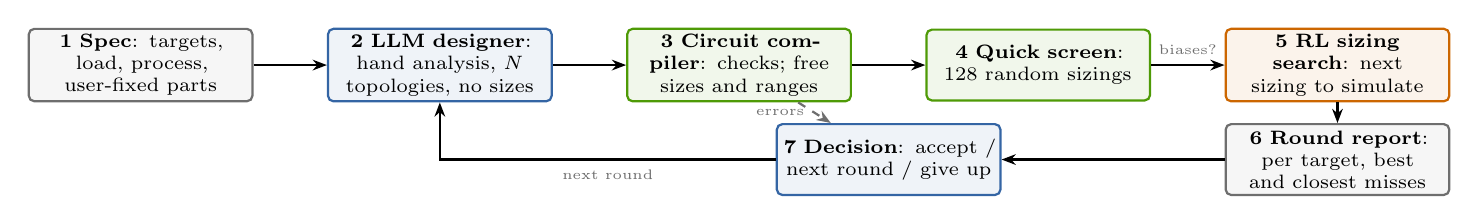
\begin{tikzpicture}[x=38mm, y=12mm]
  \node[iobox]  (spec)   at (0, 0) {\textbf{1 Spec}: targets, load, process, user-fixed parts};
  \node[llmbox] (llm)    at (1, 0) {\textbf{2 LLM designer}: hand analysis, $N$ topologies, no sizes};
  \node[simbox] (comp)   at (2, 0) {\textbf{3 Circuit compiler}: checks; free sizes and ranges};
  \node[simbox] (screen) at (3, 0) {\textbf{4 Quick screen}: 128 random sizings};
  \node[rlbox]  (rl)     at (4, 0) {\textbf{5 RL sizing search}: next sizing to simulate};
  \node[iobox]  (report) at (4, -1) {\textbf{6 Round report}: per target, best and closest misses};
  \node[llmbox] (call)   at (2.5, -1) {\textbf{7 Decision}: accept / next round / give up};
  \draw[arr] (spec) -- (llm); \draw[arr] (llm) -- (comp); \draw[arr] (comp) -- (screen);
  \draw[arr] (screen) -- node[lab, above] {biases?} (rl); \draw[arr] (rl) -- (report);
  \draw[arr] (report) -- (call);
  \draw[arr] (call) -| node[lab, pos=0.25, below] {next round} (llm);
  \draw[arr, dashed, grey] (comp) -- node[lab, left, pos=0.5] {errors} (call);
\end{tikzpicture}
\end{center}
\vspace{-4pt}
Each part does what it is reliable at. The LLM brings circuit knowledge but never gives a transistor size; it
proposes catalogue circuits or new ones as a \emph{generic circuit} (devices, connections, roles, required regions).
The compiler (fixed, not learned) checks it (complete, every net driven at DC, voltage ratings, not a copy of a test
circuit) and writes it for one process from a kit record, so any proposal runs like a catalogue circuit; device
limits come from the kit, never from the LLM. The simulator is the only judge: a topology is accepted only on a
simulated design meeting every target, and ``not found'' after $R$ rounds of $N$ topologies (default 3 and 3) does
not mean impossible. The \textbf{rule baseline} makes the same call by trying eligible catalogue circuits fewest
devices first. \textbf{Process visibility:} for open processes the LLM sees the name and public first-order numbers;
for a licensed kit (TSMC 65\,nm) only the name, and no kit data leaves the licensed machine. The explorer sees only
normalized features of candidates and their simulated results.

\textbf{The LLM harness.} Each round the model gets a fixed system prompt (its role, the evidence rule, the reply
format) and a turn with: the specification under a neutral label (task names would reveal the source circuit), $N$
and $R$, the process's public first-order numbers (open processes only), the catalogue of 20 circuits (one line each:
what it is, its device count, which metrics it measures), a table of design moves (cascode, fold, add a stage,
\dots), the netlists in play, and the last round report in a fixed layout (per topology: compiler verdict, screen,
search; per target: best value reached and closest miss). The reply has tagged sections: \texttt{<analysis>} (reading
of the spec, bias, supply, gain and bandwidth estimates, plan), one \texttt{<circuit>} per new topology (the generic
circuit), \texttt{<analyses>} (the targets restated in fixed metric names; with \texttt{<circuit>}, the only parts
the compiler reads) and an \texttt{<action>}: propose $N$ topologies, accept a circuit, or reject (refused before
round $R$). A parser checks every part; an invalid reply goes back with its errors, once, and refusals are counted
apart. In exploration mode the model also has two tools: a free compiler check, and a single-point simulation at a
sizing it chooses (at most 6 per round). Every simulation (screen, search, tool) counts against a hard budget. Keys
come from the environment, licensed processes are refused, and replies are cached so runs replay exactly.

% ==================================================================
\section{The graph model: why it was added, and why it was removed}\label{sec:gnn}

\textbf{Added} as the proposal's optional model to predict feasibility from circuit structure: to pick a topology,
reject unreachable specs and seed the policy. As a feasibility prior it ranked designs on a held-out topology with
zero-shot AUC 0.74--0.84 from the netlist and above 0.99 with operating-point and device features; as the starting
map of GP level-set (10 seeds, 600 simulations) it raised IoU on the differential pair (1\% feasible) from 0.17 to
0.92 (development results). It later served as a circuit encoder for the policy and as a critic for the LLM.
\textbf{Removed} (2026-10-27) after two leave-one-circuit-out tests on the 15 capacitor-free circuits.
\emph{Ranking topologies:} quick screens needed to reach a circuit that meets the spec (400 specs) were 4.3 for
random order, 2.5 for fewest devices first, 2.3 for the GNN, and 1.3 with perfect knowledge, so counting devices gives
nearly all the gain and the GNN saves 0.2 screens ($\approx$25 simulations). \emph{Predicting metrics:} a GP on 32 of
a circuit's own simulations beat a GNN trained on the other 14 circuits (rank correlation 0.83/0.95/0.99 vs
0.57/0.79/0.64 for gain/bandwidth/power), even after fine-tuning. With 20 circuits there is too little to learn from (Section~\ref{sec:future}); the
compiler and the quick screen now answer its questions by simulation.

% ==================================================================
\section{Preliminary results: the RL explorer}\label{sec:rl}

\textbf{Setup.} Validation is every training task of three circuits never trained on (82 achievable, 42
infeasible); test adds three held-out circuits, unseen 3-knob grids and two new topologies (411 achievable, 211
infeasible). Each episode starts from 2 designs per knob; each step offers 32 candidates per knob, drawn by a
\emph{candidate setting} (\texttt{sobol32pk}: evenly spread; \texttt{spread\_local32pk}: half near the best design so
far), described by features of a GP belief per constraint. \emph{Greedy} is a fixed rule, not RL: it picks the
candidate with the highest believed chance of meeting the spec (the probability-of-feasibility acquisition of
constrained BO); a policy with weight 1 on that feature and 0 on the rest is greedy, so the RL policy can represent it. DQN (Hungyu; pull request under review): one model per setting, 3 training
seeds, 200k steps, 6.9k parameters, untuned. Mean simulations to the first meeting design (achievable tasks, over 3
budgets and 10 seeds; none found counts budget\,+\,1), 95\% bootstrap intervals over tasks:

\begin{center}\small
\begin{tabular}{lcc@{\hspace{10pt}}cc@{\hspace{10pt}}ccc}
\toprule
& \multicolumn{2}{c}{Validation (82)} & \multicolumn{2}{c}{Test (411)} & \multicolumn{3}{c}{Test by kind: first hit} \\
\cmidrule(lr){2-3}\cmidrule(lr){4-5}\cmidrule(lr){6-8}
Method & First hit & Solved & First hit & Solved & Train circ. & Held-out circ. & New topol. \\
\midrule
Greedy (\texttt{spread\_local32pk}) & 6.4 [4.8, 8.3] & 98\% & 9.2 [7.6, 11.0] & 92\% & 6.6 & 13.6 & 12.2 \\
DQN (\texttt{spread\_local32pk}) & 7.5 [5.6, 9.6] & 96\% & 9.0 [7.5, 10.5] & 92\% & 6.5 & 13.1 & 11.2 \\
DQN (\texttt{sobol32pk}) & 8.7 [6.2, 11.5] & 94\% & 9.9 [8.4, 11.6] & 89\% & & & \\
GP level-set & 19.6 [14.5, 24.9] & 85\% & 18.1 [15.8, 20.6] & 77\% & 14.4 & 24.5 & 20.9 \\
NSGA-II & 22.0 [16.8, 27.9] & 78\% & 17.6 [15.7, 19.6] & 74\% & 15.1 & 21.8 & 19.1 \\
MAP-Elites & 25.5 [19.5, 31.7] & 73\% & 19.4 [17.2, 21.6] & 71\% & 16.4 & 24.2 & 22.0 \\
Random & 27.4 [20.6, 34.9] & 72\% & 22.6 [19.9, 25.4] & 66\% & 19.7 & 28.0 & 24.2 \\
\bottomrule
\end{tabular}
\end{center}
\vspace{-3pt}
\begin{itemize}
  \item Picking among offered candidates by a GP belief, learned or greedy, needs about half the simulations of every
  baseline and solves at least 15 points more tasks, including on held-out circuits and new topologies. Since greedy
  learns nothing, this gain belongs to the environment (offered candidates, a GP per constraint), not to RL; RL's
  contribution is only its margin over greedy.
  \item The learned DQN does not beat greedy yet: level on test (paired differences inside their 95\% intervals at
  every level), worse on validation, mostly on tight specs (19.5 vs 16.2). Greedy is strong because the belief already
  carries most of what matters; beating it is the RL question for the final report.
  \item Infeasible specs: the map's highest chance on unsimulated designs separates achievable from infeasible test
  tasks with AUROC 0.83--0.96 for DQN vs 0.73 for greedy, but random pick also reaches 0.91, so this does not yet show
  skill.
\end{itemize}

% ==================================================================
\section{Preliminary results: the LLM designer}\label{sec:llm}

\textbf{Rule baseline} (stored 512-design pools, screen 128 + search 200 per topology; 258 training specs $\times$ 10
seeds): 76\% accepts, never wrong by construction; wrong ``not found'' on 13.6\% of achievable specs (21\% of tight),
mostly because the meeting circuit lies beyond the first nine tried; median 384 simulations to accept, 2,952 to give
up. \textbf{LLM vs rules}, same stored checks, catalogue circuits only, 50 level-stratified specs per seed, specs
shown under neutral labels:

\begin{center}\small
\begin{tabular}{lcccc@{\hspace{14pt}}cccc}
\toprule
& \multicolumn{4}{c}{Seed 0 (40 achievable)} & \multicolumn{4}{c}{Seed 1 (43 achievable)} \\
\cmidrule(lr){2-5}\cmidrule(lr){6-9}
Designer & Accepts & Wrong n.f. & Sims & Found/lost & Accepts & Wrong n.f. & Sims & Found/lost \\
\midrule
Rules (fewest devices first) & 70\% & 5 & 1.00$\times$ & -- & 74\% & 6 & 1.00$\times$ & -- \\
Claude Haiku 4.5 & 74\% & 3 & 0.94$\times$ & 4 / 2 & 78\% & 4 & 0.92$\times$ & 5 / 3 \\
Claude Sonnet 5 & 78\% & 1 & 0.87$\times$ & 4 / 0 & 84\% & 1 & 0.88$\times$ & 5 / 0 \\
\bottomrule
\end{tabular}
\end{center}
\vspace{-3pt}
``Found / lost'': specs met where the rules gave up, and the reverse. Over both seeds Sonnet found 9 and lost none
(sign test $p = 0.004$); Haiku found 9 and lost 5 ($p = 0.42$). No wrong accepts. Claude Opus refused every call
with the designer's instructions and is not reported. \textbf{New topologies} (Sonnet with a compiler check and one-point simulations as tools; a stand-in compiler and
random search). With \texttt{miller2} hidden, Sonnet met two of the three specs only it meets, in two runs, with
uncompensated two-stage circuits it drew (no phase-margin target yet). The third, met by 1 in 512 \texttt{miller2}
sizings, the stand-in search misses even on \texttt{miller2} itself (0 of 1,128).

% ==================================================================
\section{Revised goals for the final report}

\begin{itemize}
  \item \textbf{RL:} PPO under the same protocol; PPO vs DQN chosen on validation by the rule fixed in advance;
  tuning ($\le$8 trials); the discount-0 ablation; beat greedy, especially on tight specs; live test on fresh designs;
  cross-process transfer to GF\,180\,nm against a warm-started GP.
  \item \textbf{Design loop:} the compiler for generic circuits; the full loop on live simulation with the trained
  explorer as the search; new topologies on held-out specs; a local model fine-tuned for topology suggestion only,
  on 341 public amplifier netlists with bias generators added; user constraints; TSMC 65\,nm with the process name only.
\end{itemize}
\textbf{Proposal feedback, addressed:} nominal corner only; prior work corrected (Section~\ref{sec:related}); scalable
ground truth; RL isolated by greedy and GP baselines; reward and belief defined; 10 seeds, 95\% intervals.

% ==================================================================
\section{Future plans: a topology-aware explorer}\label{sec:future}

The explorer learns a topology only through its own simulations, and its cost to the first meeting design doubles
from training to held-out circuits (6.5 to 13). Topology awareness needs no separate prior (PPO can train a circuit
encoder inside its network); what limits it is data: an encoder trained on 14 circuits would recognize them, not
generalize. Three levels, each kept only if it helps on held-out circuits, after the policy beats greedy without
context: (1)~\emph{in-context}: episode-history features, so the policy infers the kind of circuit from its
first simulations; (2)~\emph{hand-made context}: device count, stack depth and stages from the compiler, and the role
and required region of the device that limits (``the tail is limiting'' means the same on every circuit); (3)~a
\emph{learned graph encoder} trained end to end, only with hundreds of training topologies, compared with (2) on the
same data. The topologies would come from applying the design moves (cascode, fold, add a stage, swap device type, degenerate)
once or twice to the catalogue circuits (a few hundred, reproducibly) and from circuits the LLM proposes; each passes
the compiler (duplicates and test-circuit copies removed) and the quick screen, and trains live on the simulator.

\newpage
\begin{thebibliography}{99}\small\setlength{\itemsep}{0pt}
\bibitem{autockt} K.~Settaluri et al., ``AutoCkt: deep reinforcement learning of analog circuit designs,'' DATE, 2020.
\bibitem{ppaas} S.~Kim et al., ``PPAAS: PVT and Pareto aware analog sizing via goal-conditioned reinforcement learning,'' arXiv:2507.17003, 2025.
\bibitem{gcnrl} H.~Wang et al., ``GCN-RL circuit designer: transferable transistor sizing with graph neural networks and reinforcement learning,'' DAC, 2020.
\bibitem{metabo} M.~Volpp et al., ``Meta-learning acquisition functions for transfer learning in Bayesian optimization,'' ICLR, 2020.
\bibitem{debernardinis} F.~De Bernardinis, M.~I.~Jordan, A.~Sangiovanni-Vincentelli, ``Support vector machines for analog circuit performance representation,'' DAC, 2003.
\bibitem{linli} H.~Lin, P.~Li, ``Circuit performance classification with active learning guided sampling for support vector machines,'' IEEE TCAD 34(9), 2015.
\bibitem{zhang22} L.~Zhang et al., ``Bayesian deep active learning for analog circuit performance classification,'' ISCAS, 2022.
\bibitem{gotovos} A.~Gotovos, N.~Casati, G.~Hitz, A.~Krause, ``Active learning for level set estimation,'' IJCAI, 2013.
\bibitem{mojitor} T.~McConaghy et al., ``Variation-aware structural synthesis of analog circuits via hierarchical building blocks and structural homotopy'' (MOJITO-R), IEEE TCAD, 2009.
\bibitem{cktgnn} Z.~Dong et al., ``CktGNN: circuit graph neural network for electronic design automation,'' ICLR, 2023.
\bibitem{wusavidis} Z.~Wu, I.~Savidis, ``Transfer of performance models across analog circuit topologies with graph neural networks,'' MLCAD, 2022.
\bibitem{analogcoder} Y.~Lai et al., ``AnalogCoder: analog circuit design via training-free code generation,'' AAAI, 2025.
\bibitem{analogcoderpro} Y.~Lai et al., ``AnalogCoder-Pro: unifying analog circuit generation and optimization via multi-modal LLMs,'' arXiv:2508.02518, 2025.
\bibitem{adollm} Y.~Yin et al., ``ADO-LLM: analog design Bayesian optimization with in-context learning of large language models,'' ICCAD, 2024.
\bibitem{analogxpert} H.~Zhang et al., ``AnalogXpert: automating analog topology synthesis by incorporating circuit design expertise into large language models,'' arXiv:2412.19824, 2024.
\bibitem{eesizer} C.~Liu, D.~Chitnis, ``EEsizer: LLM-based AI agent for sizing of analog and mixed signal circuit,'' arXiv:2509.25510, 2025.
\bibitem{analogsage} Z.~Wang et al., ``AnalogSAGE: self-evolving analog design multi-agents with stratified memory and grounded experience,'' arXiv:2512.22435, 2025.
\end{thebibliography}

\end{document}
